%% §3 — Rough Surface Contact  (4 slides)
\section{Rough Surface Contact}

%% ── Slide 10: Real surfaces are rough ───────────────────────────────────────
\begin{frame}{Real Surfaces are Multi-Scale Rough}
\begin{columns}[T]
\begin{column}{0.50\textwidth}
  \textbf{Self-affine surfaces}: statistically scale-invariant
  \[
    C(q) \sim q^{-2(1+H)},\quad H\in(0,1)
  \]
  ($H$ = Hurst exponent, $q$ = spatial frequency)

  \vspace{0.5em}
  Profile sketch (three-scale superposition):
  \vspace{0.2em}

  \begin{tikzpicture}[scale=0.88]
    \begin{axis}[
      width=7cm, height=3.2cm,
      axis lines=left,
      xlabel={position $x$}, ylabel={height $h$},
      xtick=\empty, ytick=\empty,
      label style={font=\small},
      clip=false,
    ]
    \addplot[domain=0:10,samples=400,thick,mblue]
      {0.55*sin(deg(x)) + 0.22*sin(3*deg(x)) + 0.10*sin(8*deg(x))
       + 0.04*sin(18*deg(x))};
    \end{axis}
  \end{tikzpicture}
\end{column}
\begin{column}{0.46\textwidth}
  \centering
  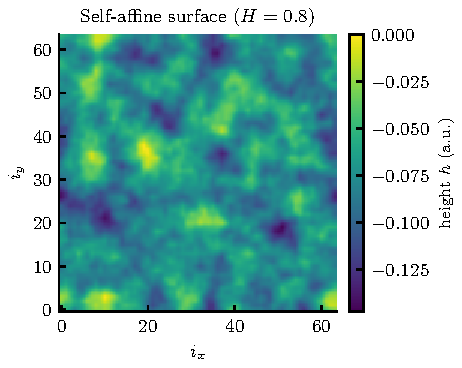
\includegraphics[width=0.94\linewidth]{figures/fig_surface.pdf}

  \vspace{0.3em}
  {\small $N_s=64$, $H=0.8$, seed 12345\\
  normalised: RMS slope $= 1$}
\end{column}
\end{columns}
\end{frame}

%% ── Slide 11: Contact problem as QP ────────────────────────────────────────
\begin{frame}{Normal Contact as a Quadratic Programme}
\begin{columns}[T]
\begin{column}{0.50\textwidth}
  \textbf{Influence matrix}: $u = Sp$, symmetric PSD ($N\!\times\!N$)

  \textbf{Complementarity energy}:
  \[
    W(p) = \frac{1}{2}p^\T S p + p^\T g_0
  \]

  \textbf{Minimise} subject to:
  \[
    p_i \ge 0 \quad\forall i, \qquad
    \frac{1}{N}\sum_i p_i = \pbar
  \]

  \vspace{0.3em}
  \textbf{KKT conditions} (complementarity):
  \[
    (Sp+g_0)_i \ge 0,\quad p_i \ge 0
  \]
  \[
    p_i\,(Sp+g_0)_i = 0
  \]
\end{column}
\begin{column}{0.46\textwidth}
  \begin{block}{Physical meaning}
    \begin{itemize}
      \item $p_i > 0$: element \emph{in contact}
        $\Rightarrow$ gap $= 0$
      \item $p_i = 0$: element \emph{not in contact}
        $\Rightarrow$ gap $\ge 0$
    \end{itemize}
  \end{block}
  \vspace{0.4em}
  \begin{alertblock}{No-penetration + non-adhesion}
    $g_i = u_i + g_{0,i} - \delta \ge 0$ everywhere,\\
    with $\delta$ the rigid-body approach.
  \end{alertblock}
\end{column}
\end{columns}
\end{frame}

%% ── Slide 12: Full Polonsky–Keer algorithm ──────────────────────────────────
\begin{frame}{Polonsky--Keer Projected CG (full)}
\begin{columns}[T]
\begin{column}{0.50\textwidth}
  \begin{block}{Initialisation}
    $p \leftarrow \pbar\mathbf{1}$;\quad
    $u \leftarrow Sp$;\quad
    $r \leftarrow u + g_0$
  \end{block}
  \begin{block}{Iteration ($k=1,\ldots$)}
    1. Shift gradient:
    $\bar r \leftarrow r - \langle r\rangle_{\mathcal{C}}$
    \par 2. Suppress: $r_i \leftarrow 0$ if $p_i=0$ and $\bar r_i \ge 0$
    \par 3. $\delta \leftarrow \|r\|^2$;\quad
      \textbf{converge} if $\delta < \varepsilon^2\delta_0$
    \par 4. CG direction: $t \leftarrow r + \tfrac{\delta}{\delta_{\rm prev}}\,t$
      (masked)
    \par 5. Line search: $\tau = \delta\,/\,\langle t,St\rangle_{\mathcal{C}}$
    \par 6. Update: $p \leftarrow \max(p - \tau t, 0)$
    \par 7. Overlap: $p_i \mathrel{-}= \tau g_i$ if $p_i=0,\,g_i<0$
    \par 8. Normalise: $p \leftarrow p\cdot\pbar N/\textstyle\sum p$
    \par 9. Recompute $u = Sp$;\; $r = u + g_0$
  \end{block}
\end{column}
\begin{column}{0.46\textwidth}
  \begin{block}{Convergence criterion}
    \[
      E_k = \frac{\sum_i p_i |g_i|}{N\,\pbar\,\Delta g}
      \;<\;\varepsilon
    \]
  \end{block}
  \vspace{0.4em}
  \begin{itemize}
    \item \textbf{Two H-matvecs per step}:\\
      one for gradient update,\\
      one for the line search
    \item Overlap correction resets CG
      ($\delta/\delta_{\rm prev}\leftarrow 0$)
    \item Converges in $\lesssim 30$ iterations
      for typical rough surfaces at
      $\pbar=0.05\,\Esta$
  \end{itemize}
\end{column}
\end{columns}
\end{frame}

%% ── Slide 13: Rough contact result ──────────────────────────────────────────
\begin{frame}{Rough Surface Contact Result ($N_s=64$, $\pbar=0.05$)}
  \centering
  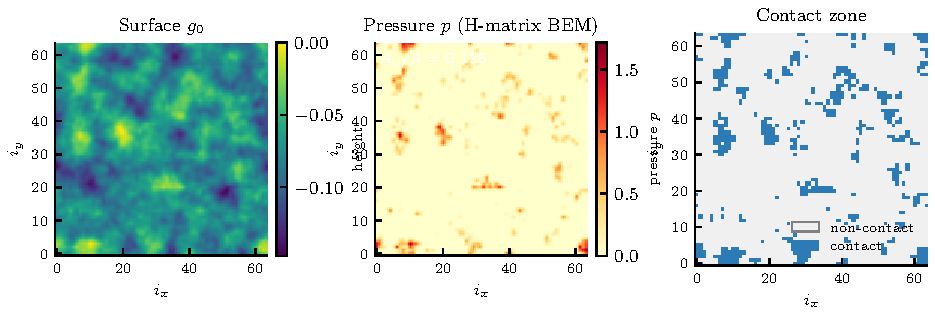
\includegraphics[width=0.96\linewidth]{figures/fig_rough_result.pdf}
  \vspace{0.2em}

  \begin{columns}
  \begin{column}{0.32\textwidth}
    \centering{\small Self-affine surface ($H=0.8$)}
  \end{column}
  \begin{column}{0.32\textwidth}
    \centering{\small $A_c/A = 0.126$,\; mean $p = 0.05\,\Esta$}
  \end{column}
  \begin{column}{0.32\textwidth}
    \centering{\small Contact in 12.6\,\% of elements}
  \end{column}
  \end{columns}
\end{frame}
